\documentclass[convert]{standalone}


\usepackage{tikz}
\usepackage{ifthen}

\tikzstyle{dots}=[%
	every node/.style={
		circle, inner sep = 0, fill=black, minimum size = 3pt, anchor=south
	}%
]

\begin{document}
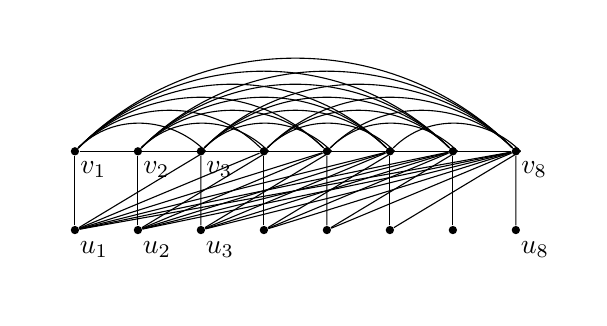
\begin{tikzpicture}[scale=0.2, dots]
	\draw[fill=white, draw=none] (1,-4) rectangle (36,9);

	\node[label = {[label distance=2pt] below right:{$v_1$}}] (v1) at ( 4,5) {};
	\node[label = {[label distance=2pt] below right:{$v_2$}}] (v2) at ( 8,5) {};
	\node[label = {[label distance=2pt] below right:{$v_3$}}] (v3) at (12,5) {};
	\node (v4) at (16,5) {};
	\node (v5) at (20,5) {};
	\node (v6) at (24,5) {};
	\node (v7) at (28,5) {};
	\node[label = {[label distance=2pt] below right:{$v_8$}}] (v8) at (32,5) {};

	\node[label = {[label distance=2pt] below right:{$u_1$}}] (u1) at ( 4,0) {};
	\node[label = {[label distance=2pt] below right:{$u_2$}}] (u2) at ( 8,0) {};
	\node[label = {[label distance=2pt] below right:{$u_3$}}] (u3) at (12,0) {};
	\node (u4) at (16,0) {};
	\node (u5) at (20,0) {};
	\node (u6) at (24,0) {};
	\node (u7) at (28,0) {};
	\node[label = {[label distance=2pt] below right:{$u_8$}}] (u8) at (32,0) {};

	\foreach \x in {1,...,6} {
		\draw (u\x) -- (v\x);
		\pgfmathsetmacro\ystart{\x+2};
		\foreach \y in {\ystart,...,8} {
			\draw (u\x) -- (v\y);
		};
	};
	\draw (u7) -- (v7);
	\draw (u8) -- (v8);

	\foreach \x in {1,...,6} {
		\pgfmathsetmacro\ypp{\x+1};
		\draw (v\x) -- (v\ypp);
		\pgfmathsetmacro\ystart{\ypp+1};
		\foreach \y in {\ystart,...,8} {
			\draw (v\x) to [in=135, out=45] (v\y);
		};
	}
	\draw (v7) -- (v8);
\end{tikzpicture}
\end{document}








